\chapter{Smooth Manifolds}
A topological space $X$ has a countable topological base, when there exists a
countable system of open sets $V = \{U_i\big| i\in \NN\}$, such that every open set can be
written in the form $\cup_{i\in I}U_i$, where $I\sseq\NN$.

For instance $\RR^n$ has a countable basis for the topology given by
\begin{align*}
  \C{V} = \{\mrg{D}\big| x=(x_1, \cdots, x_n), x_i\in \QQ; \epsilon\in\QQ, \epsilon>0\}
\end{align*}

where $\mrg{D}(x;\epsilon)$ is the open ball with center at $x$ and radius $\epsilon$.
A topological space $X$ is a Hausdorff space when, for arbitrary distinct $x,y\in X$,
there exist open neighborhoods $U_x$ and $U_y$ with $U_x\cap u_y=\ns$.

\begin{definition}\label{def:8-1}
  A topological manifold $M$ is a topological Hausdorff space that
  has a countable basis for its topology and that is locally homeomorphic to $\RR^n$.
  The number $n$ is called the dimension of $M$.
\end{definition}

\begin{remark}\label{remark:8-2}
  Every open ball $\mrg{D}^n(0, \epsilon)$ in $\RR^n$ is diffeomorphic to $\RR^n$ via the map
  $\Phi$, given by
  \begin{align*}
    \Phi(y) = \left\{\begin{aligned}
      & \tan(\pi\|y\|/2\epsilon)\cdot y/\|y\| && \text{ if } y\neq 0, \|y\|<\epsilon \\
      & 0 && \text{ if } y = 0
    \end{aligned}\right.
  \end{align*}

  (Smoothness of $\Phi$ and $\Phi^{-1}$ at 0 can be shown by means of the Taylor series at 0
  for $\tan$ and $\arctan$.) Thus in Definition \ref{def:8-1} it does not matter whether we require
  that $M^n$ is locally homeomorphic to $\RR^n$ or to an open set in $\RR^n$.
\end{remark}


\begin{definition}\label{def:8-3}\;\par 
  \begin{enumerate}[(i)]
    \item A chart $(U, h)$ on an $n$-dimensional manifold is a homeomorphism 
      $h:U\to U'$, where $U$ is an open set in $M$ and $U'$ is an open set in $\RR^n$.
    \item A system $A = \{h_i: U_i\to U_i'\big| i\in J\}$ of charts is called an atlas, provided 
      $\{U_i \big| i\in J\}$ covers $M$.
    \item An atlas is smooth when all of the maps 
      \begin{align*}
        h_{ji} = h_j\circ h_i^{-1}:h_i(U_i\cap U_j) \to h_j(U_i\cap U_j)
      \end{align*}
      are smooth. They are called chart transformations (or transition functions) for the given atlas.
  \end{enumerate}
\end{definition}

Note in Definition \ref{def:8-3}.(iii) that $h_i(U_i\cap U_j)$ is open in $\RR^n$.
Two smooth atlases $A_1, A_2$ are smoothly equivalent if $A_1\cup A_2$ is a smooth atlas.
This defines an equivalence relation on the set of atlases on $M$. A smooth structure
on $M$ is an equivalence class $\C{A}$ of smooth atlases on $M$.

\begin{definition}\label{def:8-4}
  A smooth manifold is a pair $(M, \C{A})$ consisting of a topological
manifold $M$ and a smooth structure $\C{A}$ on $M$.
\end{definition}

Usually $\C{A}$ is suppressed from the notation and we write $M$ instead of $(M, \C{A})$. 

\begin{example}\label{example:8-5}
  The $n$-dimensional sphere $S^n = \{x\in\RR^{n+1}\big| \|x\|=1\}$ is an $n$-dimensional smooth 
  manifold. We define an atlas with $2(n+1)$ charts $(U_{\pm i}, h_{\pm i})$ where 
  \begin{align*}
    U_{+i} = \{x\in S^n\big| x_i>0\},
    && U_{-i} = \{x\in S^n\big| x_i<0\}
  \end{align*}

  and $h_{\pm i}:U_{\pm i}\to \mrg{D}^n$ is the map given by $h_{\pm i}(x) = (x_1, \cdots, \hat{x}_i, \cdots, x_{n+1})$. 
  The circumflex over $x_i$ denotes that $x_i$ is omitted. The inverse map is 
  \begin{align*}
    h_{\pm i}^{-1}(u) = \left(u_1, \cdots, u_{i-1}, \pm\sqrt{1-\|u\|^2}, u_i, \cdots, u_n\right)
  \end{align*}
  It is left to the reader to prove that the chart transformations are smooth.
\end{example}

\begin{example}[The projective space $\RR\B{P}^n$]\label{example:8-6}\index{projective space}
  On $S^n$ we define an equivalence relation:
  \begin{align*}
    x\sim y \equ x = y \text{ or } x = -y
  \end{align*}
  The equivalence classes $[x] = \{x, -x\}$ define the set $\RR\B{P}^n$. Alternatively one can
  consider $\RR\B{P}^n$ as all lines in $\RR^{n+1}$ through 0. Let 1r be the canonical projection
  \begin{align*}
    \pi:S^n\to \RR\B{P}^n; && \pi(x) = [x].
  \end{align*}

  We give $\RR\B{P}^n$ the quotient topology, i.e.
  \begin{align*}
    U\sseq \RR\B{P}^n \text{ open } \equ \pi^{-1}(U)\sseq S^n \text{ open }.
  \end{align*}
  With the conventions of Example \ref{example:8-5}, $\pi(U_{-i}) = \pi(U_{+i})$. We define 
  $U_i = \pi_{\pm i}\sseq \RR\B{P}^n$, and note that $\pi^{-1}(U_i) = U_{+i}\cup U_{-i}$ with 
  $U_{+i}\cap U_{-i}=\ns$. An equivalence calss $[x]\in U_i$ has one representive in $U_{+i}$ and 
  one representive in $U_{-i}$. Hence $\pi:U_{+i}\to U_{-i}$ is a homeomorphism. We define
  \begin{align*}
    h_i = h_{+i}\circ \pi^{-1}:U_i\to\mrg{D}^n,
  \end{align*}
  $i=1, \cdots, n$. This gives a smooth atlas on $\RR\B{P}^n$.
\end{example}

\begin{definition}\label{def:8-7}
  Consider smooth manifolds $M_1$ and $M_2$ and a continuous map $f: M_1\to M_2$.
  The map $f$ is called smooth at $x\in M_1$ if there exist charts
  $h_1:U_1\to U_1'$ and $h_2:U_2\to U_2'$ on $M_1$ and $M_2$ with $x\in U_1$ and $f(x)\in U_2$,
  such that
  \begin{align*}
    h_2\circ f\circ h_1^{-1}:h_1(f^{-1}(U_2))\to U_2'
  \end{align*}
  is smooth in a neighborhood of $h_1(x)$. If $f$ is smooth at all points of $M_1$ then $f$ is said 
  to be smooth.
\end{definition}

Since chart transformations (by Definition \ref{def:8-3}.(iii)) are smooth, we have that
Definition \ref{def:8-7} is independent of the choice of charts in the given atlases for $M_1$
and $M_2$. A composition of two smooth maps is smooth. 

A \Index{diffeomorphism} $f: M_1\to M_2$ between smooth manifolds is a smooth map that
has a smooth inverse. In particular a diffeomorphism is a homeomorphism.
As soon as we have chosen an atlas $\C{A}$ on a manifold $M$, we know which functions
on M are smooth. In particular we know when a homeomorphism $f:V\to V'$
between an open set $V\subset M$ and an open set $V'\subseteq \RR^n$ is a diffeomorphism.
We can therefore define a new \Index{maximal atlas}, $\C{A}_{\max}$, associated with the given
smooth structure:
\begin{align*}
  \C{A}_{\max} = \{
      f:V \to V'\big| 
        V \sseq M^n \text{ open }, 
        V'\sseq\RR^n \text{ open }, 
        f \text{ diffeomorphism }
    \}.
\end{align*}

The inverse diffeomorphisms $f^{-1}: V'\to V$ will be called local parametrizations.
From Remark \ref{remark:8-2} it follows that every point in a smooth manifold $M^n$ has an
open neighborhood $V\sseq M^n$ that is diffeomorphic to $\RR^n$.

From now on chart will mean a chart in the maximal atlas.

\begin{definition}\label{def:8-8}
  A subset $N\subset M^n$ of a smooth manifold is said to be a smooth
  submanifold (of dimension $k$), if the following condition is satisfied: for every
  $x\in N$ there exists a chart $h:U\to U'$ on $M$ such that
  \begin{align}\label{eq:8-1}
    x\in U \text{ and } h(U\cap N) = U'\cap \RR^k,
  \end{align}
  where $\RR^k\sseq\RR^n$ is the standard subspace.
\end{definition}

It is easy to see that a smooth submanifold N of a smooth manifold $M$ is a smooth
manifold again. A smooth atlas on N is given by all $h:U\cap N\to U'\RR^k$, where
$(U, h)$ are charts on $M$ satisfying \eqref{eq:8-1}.

\begin{example}\label{example:8-9}
  The $n$-sphere $S^n$ is a smooth submanifold of $\RR^{n+1}$. In fact the
  charts $(U_{\pm i}, h_{\pm i})$ from Example \ref{example:8-5} can easily be extended to 
  diffeomorphisms satisfying \eqref{eq:8-1}.
\end{example}

\begin{definition}\label{def:8-10}
  An \Index{embedding} is a smooth map $f:N\to M$ such that $f(N)\subset M$
  is a smooth submanifold and $f: N\to f (N)$ is a diffeomorphism.
\end{definition}


\begin{theorem}\label{theorem:8-11}
  Let $M^n$ be a smooth manifold of dimension $n$. There exists an
  embedding of $M^n$ into a Euclidean space $\RR^{n+k}$.
\end{theorem}

This result will be proved below for a compact $M$, but let us first note that
$N^n = f(M^n)$ satisfies the following condition:

For every $p\in N^n$ there exists an open neighborhood $V\sseq\RR^{n+k}$ , an open set
$U'\sseq\RR^n$ and a homeomorphism
\begin{align*}
  g:U'\to N\cap V,
\end{align*}

such that $g$ is smooth (consider as a map from $U'$ to $V$) and such that $D_xg:\RR^n\to\RR^{n+k}$ is
injective.

This is the usual definition of an embedded manifold (regular surface when $n = 2$).
Theorem \ref{theorem:8-11} tells us that every smooth manifold is diffeomorphic to an embedded
manifold. Conversely, if $N\sseq\RR^{n+k}$ satisfies the above condition, then the implicit
function theorem shows that it is a submanifold in the sense of Definition \ref{def:8-8}.
A theorem by H. Whitney asserts that the codimension $k$ in Theorem \ref{theorem:8-11} can
always be taken to be less or equal to $n + 1$. On the other hand $k$ cannot be
arbitrarily small. $\RR\B{P}^2$ cannot be embedded in $\RR^3$.


\begin{lemma}\label{lemma:8-12}
  Let $M^n$ be an $n$-dimensional smooth manifold. For $p\in M$ there exist smooth maps
  \begin{align*}
    \phi_p:M\to \RR, && f_p:M\to \RR^n
  \end{align*}
  such that $\phi_p(p)>0$, and $f_p$ maps open set $M\to \phi_p^{-1}(0)$ diffeomorphically onto 
  an open subset  of $\RR^n$.
\end{lemma}

\begin{proof}
  Choose a chart $h: V\to V'$ with $p\in V$. By Lemma \ref{lemma:A.7} we can find a
function $\psi\in C^\infty(\RR^n, \RR)$ with compact support $\R{supp}_{\RR^n}(\psi)\sseq V'$, 
such that $\psi$ is constantly equal to 1 on an open neighborhood $U'\subset V'$ of $h(p)$.The 
smooth map $f_p$ can now be defined by
\begin{align*}
  f_p(q) = \left\{\begin{aligned}
    & \psi(h(q))h(q) && \text{ if } q\in V \\
    & 0 && \text{ otherwise }
  \end{aligned}\right.
\end{align*}
On the open neighborhood $U = h^{-1}(U')$ the function $f_p$ coincides with $h$ and
therefore maps $U$ diffeomorphically onto $U'$. Choose $\psi_0\in C^\infty(\RR^n, \RR)$ with
compact support $\R{supp}_{\RR^n}(\psi_0)\sseq U'$ and $\psi_0(h(p))>0$, and let
\begin{align*}
  \phi(q) = \left\{\begin{aligned}
    & \psi_0(h(q)) && \text{ if } q\in V \\
    & 0 && \text{ otherwise }
  \end{aligned}\right.
\end{align*}

Since $M-\phi_p^{-1}(0)\sseq U$, the final assertion holds.
\end{proof}

\noindent\textbf{Proof of Theorem \ref{theorem:8-11}} ($M$ compact)%
For every $p\in M$ choose $\phi_p$ and $f_p$ as in
Lemma \ref{lemma:8-12}. By compactness $M$ can be covered by a finite number of the sets
$M - \phi_p^{-1}(0)$. After a change of notation we have smooth functions
\begin{align*}
  \phi_j: M\to\RR, && f_j:M\to \RR^n && (1\le j\le d)
\end{align*}
satisfying the following conditions:
\begin{enumerate}[(i)]
  \item The open sets $U_j = M - \phi_j^{-1}(0)$ cover $M$.
  \item $f_{j|u_j}$ maps $U_j$ diffeomorphically onto an open set $U_j'\in\RR^n$.
\end{enumerate}
We define a smooth map $f:M\to \RR^{nd+d}$ by setting 
\begin{align*}
  f(q) = (f_1(q), \cdots, f_d(q), \phi_1(q), \cdots, \phi_d(q) ).
\end{align*}
Assuming $f(q_l) = f(q_2)$, we can by (i) choose $j$ such that $q_1\in U_j$. Then
$\phi_j(q_2)=\phi_j(q_1)\neq 0, q_2\in U_j$, and by (ii), $q_1=q_2$. Hence $f$ is injective. 
Since $M$ is compact, $f$ is a homeomorphism from $M$ to $f(M).$ Let
\begin{align*}
  \pi_1:\RR^{nd+d}\to\RR, && \pi_2:\RR^{nd+d}\to\RR^{n(d-1) + d}
\end{align*}
be the projections on the first $n$ coordinates and the last $n(d - 1) + d$ coordinates,
respectively. By (ii) $\pi_1\circ f = f_1$ is a diffeomorphism from $U_1$ to $U_1'$. In particular
$\pi_1$ maps $f(U_1)$ bijectively onto $U_1'$. Hence $f(U_1)$ is the graph of the smooth map
\begin{align*}
  g_1:U_1'\to\RR^{n(d-1)+d}; && 
  g_1 = \pi_2\circ f\circ (f_{1|U_1})^{-1}
\end{align*}
Define a diffeomorphism $h_1$ from $\pi_1^{-1}(U_1')$ to itself by the formula 
\begin{align*}
  h_1(x, y) = (x, y-g_1(x)), && x\in U_1', y\in \RR^{n(d-1)+d}.
\end{align*}
We see that $h_1$ maps $f(U_1)$ bijectively onto $U_1'\times\{0\}$. Since $f(U_1)$ is open in
$f(M), f(U_1) = f(M)\cap W_1$ for an open set $W_1\sseq \RR^{nd+d}$, which can be chosen
to be contained in $\pi_1^{-1}(U_1')$. The restriction $h_{1|W_1}$ is a diffeomorphism from $W_1$
onto an open set $W_1'$, and it maps $f(M)\cap W_1$ bijectively onto $W_1'\cap \RR^n$ , as
required by Definition \ref{def:8-8}. The remaining $f(U_j)$ are treated analogously. Hence
$f(M)$ is a smooth submanifold of $\RR^{nd+d}$. Note also that $f_{|U_1}:U_1\to f(U_1)$ is
a diffeomorphism, namely the composite of $f_{1|U_1}:U_1\to U_1'$ and the inverse to
the diffeomorphism $f(U_)\to U_1'$ induced by $\pi_1$. The remaining $U_j$ are treated
analogously. Hence $f: M\to f(M)$ is a diffeomorphism. \hfill\(\qedsymbol\)

\begin{remark}\label{remark:8-13}
  The general case of Theorem 8.11 is shown in standard text books
on differential topology. To get $k = n + 1$ (\Index{Whitney's embedding theorem})
one uses Theorem \ref{theorem:11-6} below. In the proofs above one can change ``smooth
manifold'' to "topological manifold", ``smooth map'' to ``continuous map'' and
``diffeomorphism'' to ``homeomorphism''. This will lead to the theorem below,
where the concept (locally flat) topological submanifold is defined in analogy to
Definition \ref{def:8-8}, but with a homeomorphism instead of the diffeomorphism $h$.
\end{remark}

\begin{theorem}\label{theorem:8-14}
  Every compact topological $n$-dimensional manifold is homeomorphic to a (locally flat) 
  topological submanifold of a Euclidean space $\RR^{n+k}$
\end{theorem}

On a topological manifold $M^n$ we have the $\RR$-algebra $C^0(M, \RR)$ of continuous
functions $M\to\RR$. A smooth structure $\C{A}$ on $M^n$ gives a subalgebra
\begin{align*}
  C^\infty((M, \C{A}), \RR)\sseq C^0(M, \RR)
\end{align*}

consisting of the maps $M\to \RR$, that are smooth in the structure $\C{A}$ on $M$ (and
the standard structure on $\RR$). Usually $\C{A}$ is suppressed from the notation, and the
$\RR$-algebra of smooth real-valued functions on $M$ is denoted by $C^\infty(M, \RR)$. This
subalgebra of $C^0(M, \RR)$ uniquely determines the smooth structure on $M$. This is
a consequence of the following Proposition \ref{prop:8-15} applied to the identity maps $\id_M$
\begin{align*}
  (M, \C{A}_1) \leftrightarrows (M, \C{A}_2).
\end{align*}

\begin{proposition}\label{prop:8-15}
  If $g:N\to M$ is a continuous map between smooth manifolds $N$ and $M$, then $g$ is smooth 
  if and only if the homomorphism
  \begin{align*}
    g^*:C^0(M, \RR)\to C^0(N, \RR)
  \end{align*}
  given by $g^*(\psi) = \psi\circ g$ maps $C^\infty(M, \RR)$ to $C^\infty(N, \RR)$.
\end{proposition}

\begin{proof}
  ``Only if'' follows because a composition of two smooth maps is smooth.
  Conversely if the condition on $g^*$ is satisfied, Lemma \ref{lemma:8-12} applied to $p = g(q)$
  yields a smooth map $f:M^n\to\RR^n$ and an open neighborhood $V$ of $p$ in $M$, such
  that the restriction $f_{|V}$ is a diffeomorphism of $V$ onto an open subset of $\RR^n$. For the
  $j$-th coordinate function $f_j\in C^\infty(M, \RR)$ we have $f_j\circ g = g^*(f_j)\in C^\infty(N, \RR)$,
  so that $f\circ g:N\to\RR$ is smooth. Using the chart $f_{|W}$ on $M$, $g$ is seen to be
  smooth at $q$.
\end{proof}

\begin{remark}\label{remark:8-16}
  There is a quite elaborate theory which attempts to classify $n$
  dimensional smooth and topological manifolds up to diffeomorphism and homeomorphism. 
  Every connected 1-dimensional smooth or topological manifold is diffeomorphic or homeomorphic 
  to $\RR$ or $S^1$. For $n = 2$ there is a complete classification of the compact connected 
  surfaces. There are two infinite families of them:

  \begin{figure}[!htb]
    \centering
    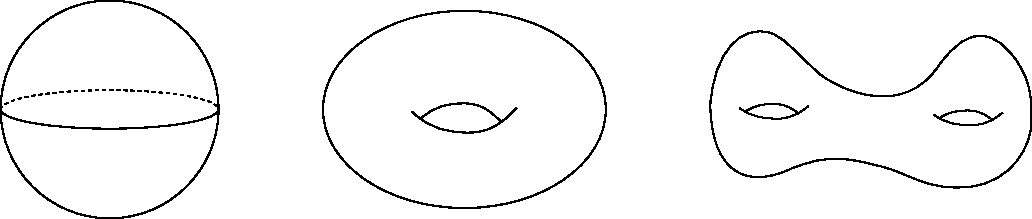
\includegraphics[width=.75\linewidth]{pics/chap8.pdf}
    \caption{Orientable surfaces}
    \label{fig:Orientable-surfaces}
  \end{figure}

  Non-orientable surfaces: $\B{RP}^2$, Klein's bottle, etc. See e.g. [Hirsch], [Massey].
  In dimension 3, one meets a famous open problem: the Poincare conjecture, which
  asserts that every compact topological 3-manifold that is homotopy equivalent to
  53 is homeomorphic to $S^3$. It is known that every topological 3-manifold $M^3$
  has a smooth structure $\C{A}$ and that two homeomorphic smooth 3-manifolds also
  are diffeomorphic. In the mid 1950s J. Milnor discovered smooth 7-manifolds
  that are homeomorphic to $S^7$, but not diffeomorphic to $S^7$. In collaboration with
  M. Kervaire he classified such exotic n-spheres. For example they showed that
  there are exactly 28 oriented diffeomorphism classes of exotic 7-spheres. In 1960
  Kervaire described a topological 10-manifold that has no smooth structure. During
  the 1960s the so-called ``surgery'' technique was developed, which in principle
  classifies all manifolds of a specified homotopy type, but only for $n\ge 5$.

  In the early 1980s M. Freedman completely classified the simply-connected compact 
  topological 4-manifolds; see [Freedman-Quinn]. At the same time S. Donaldson proved 
  some very surprising results about smooth compact 4-manifolds, which showed that there 
  is a tremendous difference between smooth and topological 4-manifolds. Donaldson used 
  methods originating in mathematical physics(Yang-Mills theory). This has led to a wealth of 
  new results on smooth 4-manifolds; see [Donaldson-Kronheimer].

  One of the most bizarre conclusions of the work of Donaldson and Freedman is
  that there exists a smooth structure on $\RR^4$ such that the resulting smooth 4-manifold
  `$`\RR^4$'' is not diffeomorphic to the usual $\RR^4$. It was proved earlier by S. Smale that
  every smooth structure on $\RR^n$ for $n\neq 4$ is diffeomorphic to the standard $\RR^n$.
\end{remark}